\chapter{Related Work}

A variety of approaches are able to locate precise object boundaries, although few directly address the problem of sidewalk segmentation in "blobby" or compact regions. 
Several tools for segmentation appear for segmenting ribbon-like features in \ac{VHR}, we list Grabcut ~\cite{Rother2004-ou}, Slic~\cite{Achanta:149300}, and Active Contours~\cite{Kass88snakes:active} as examples.
Results for these methods on a simple sidewalk are shown in \figref{fig:Method_comparison} which shows qualitative results of each method. 
We observe that grabcut had decent performance on this example, but it is still unable to identify edges in shadow or correctly determine the width of the sidewalk region in the vicinity of a driveway, which seems to be made of the same material as the sidewalk. 
In addition we observe that all three approaches recognize the gutter as part of the sidewalk because it has the camouflage texture.

\begin{figure}[H]
    \centering
    \includegraphics[width=0.55\textwidth]{Figures/compare.png}
    \caption[Method comparison with Grabcut, Active Contours, and Slic]{
        % Method comparison with Grabcut, Active contour and Slic
        A comparison between Grabcut(left), SLIC (center) and Active Contours (right) 
        on an example of a sidewalk from 6-inch aerial imagery; 
        \aclp{TP} are rendered in green, 
        \aclp{FN} are rendered in blue, and 
        \aclp{FP} are rendered in red.
        The SLIC image contains all super-pixels that intersect the initial trajectory of a walking path; the Active Contours and GrabCut methods are initialized with the SLIC results.
    }
    \label{fig:Method_comparison}
\end{figure}

\section{Image Segmentation via Grabcut} 

\begin{figure}[H]
    \centering
    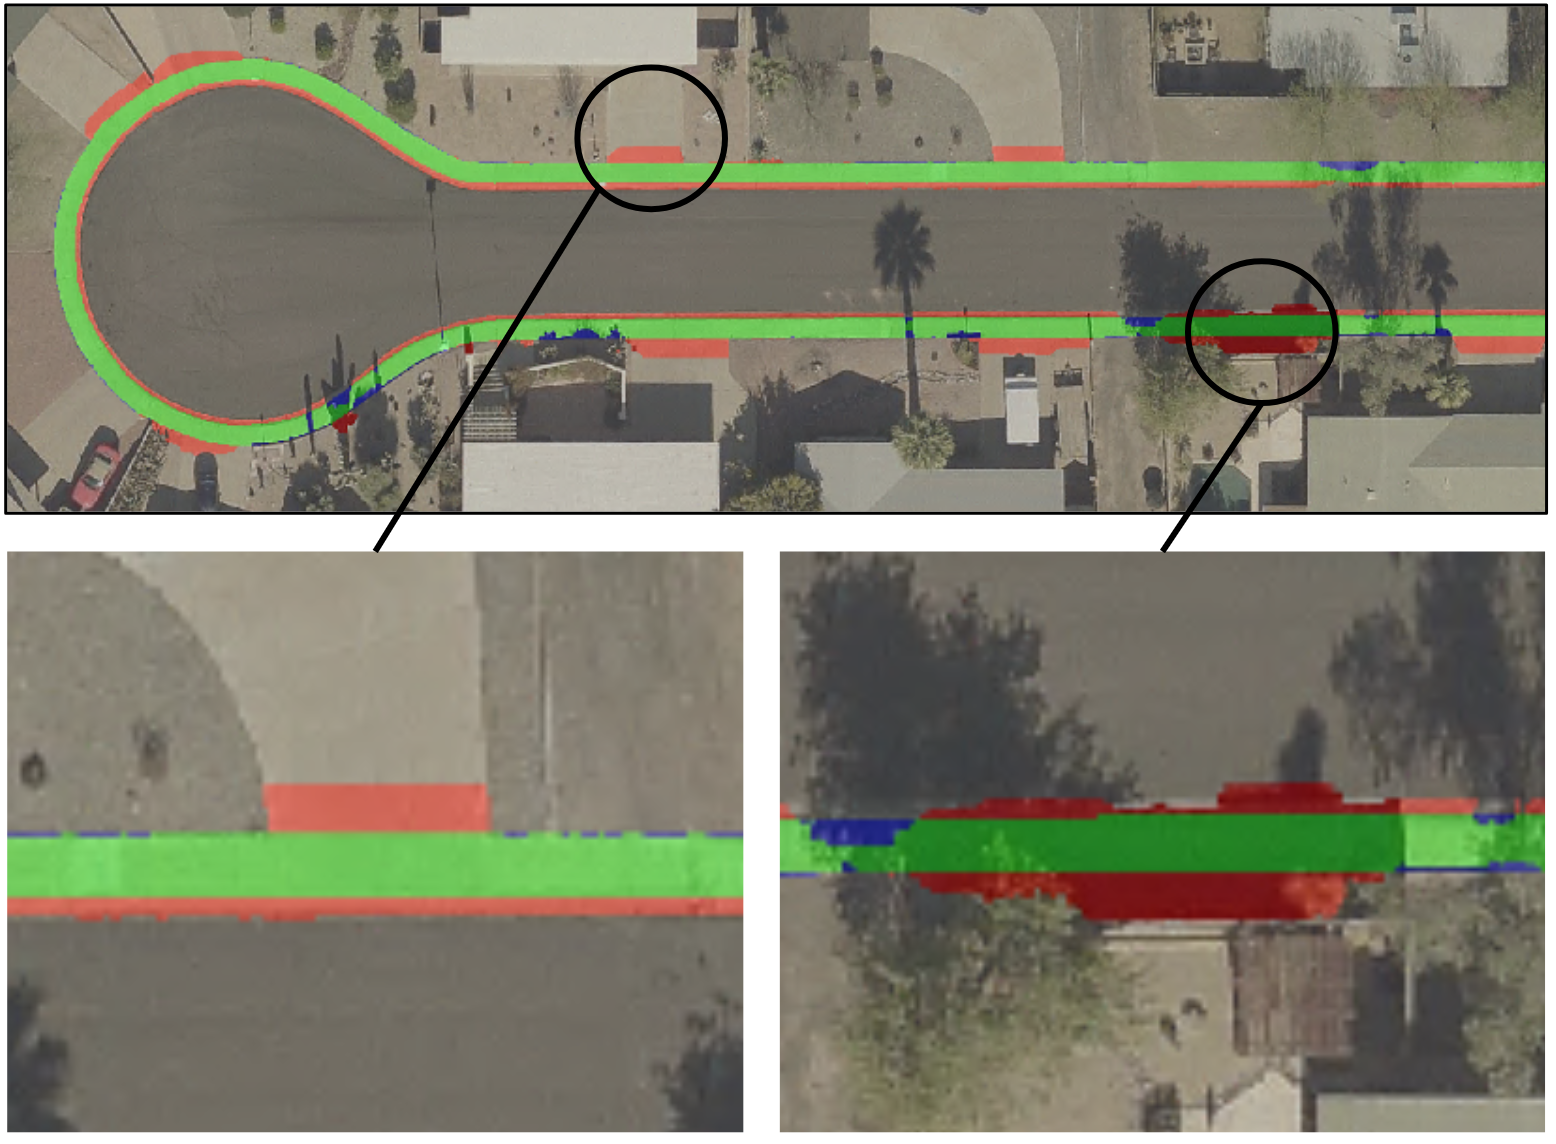
\includegraphics[width=\textwidth]{Figures/grabcut_sample.png}
    \caption[Example of Grabcut]{Detail demonstration with grabcut method. Row 2 indicates examples of false positive, which is recognized a non-sidewalk feature (shadow) and similar texture (driveway) as a part of sidewalk.}
    \label{fig:grabcut}
\end{figure}

Grabcut is a powerful image segmentation tool that combines both texture(color) and edge(contrast) information~\cite{Rother2004-ou}. 
It was designed to efficiently extract a foreground object from a complex background. 
According to figure \ref{fig:Method_comparison} and figure \ref{fig:grabcut}, the overall performance on grabcut applied to a ribbon-like feature is fairly accurate, but it's hard to identify objects above the sidewalk such as shadows, gutters or foliage. 
Grabcut seems to identify the occluded regions as negative, we suspect that is because of the lack of width control.

\section {Super-pixels and Feature Extraction with SLIC}

\begin{figure}[H]
    \centering
    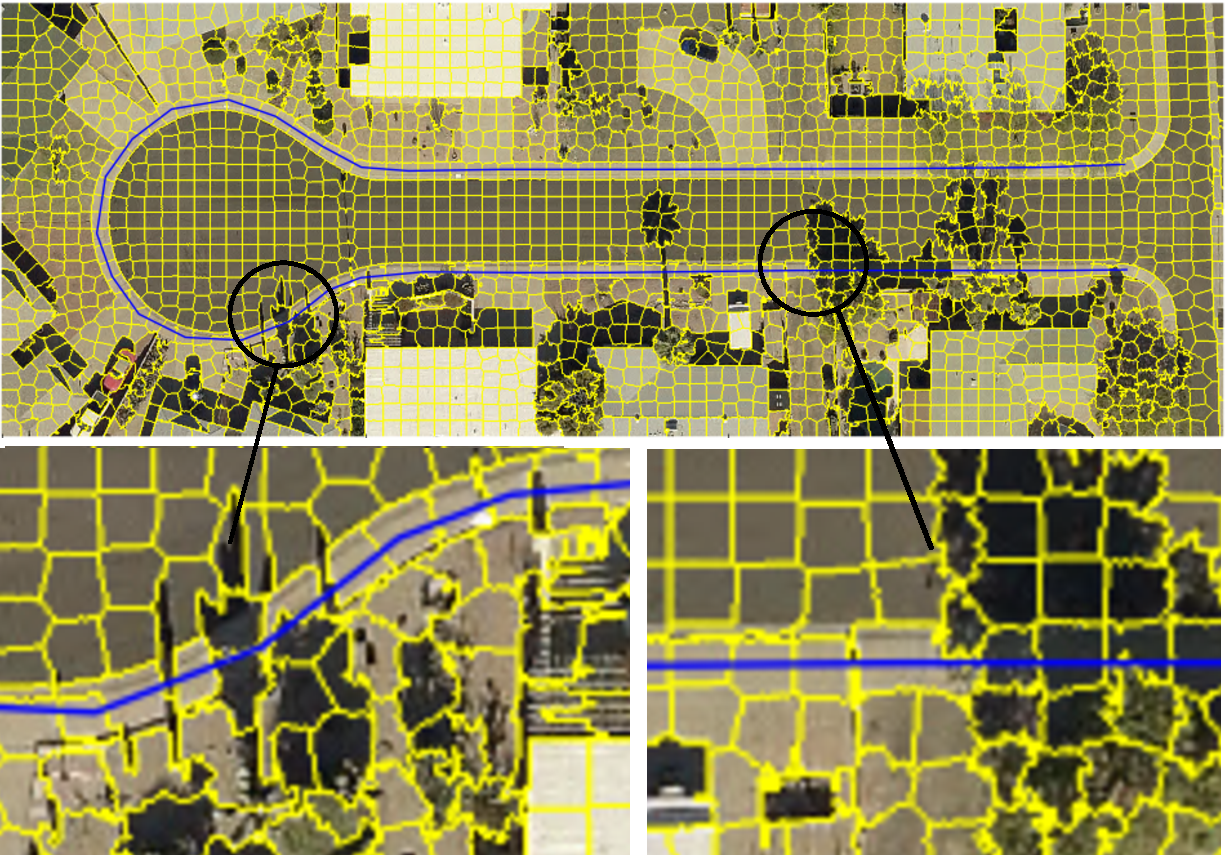
\includegraphics[width=\textwidth]{Figures/slic_sample1.pdf}
    \caption[Example of Simple Linear Iterative Clustering]{Detail demonstration on segmenting large image into irregularly shaped super-pixels with \ac{SLIC}. Row 2 indicates examples of false positive, with recognized a non-sidewalk feature (shadow) as a part of sidewalk.}
    \label{fig:slic}
\end{figure}

Simple linear iterative clustering (SLIC) works with super-pixels, which segment a large image into different irregularly shaped regions of homogeneous appearance or texture~\cite{Achanta:149300}. 
It uses the compact evenly distributed homogeneous regions of an image as a pre-processing step, so that image segmentation can be accomplished by grouping super-pixels which snap to natural boundaries in an image. 
Alternatively, super-pixels can initiate a region growing process~\cite{Borovec2017-fz}. 
As shown in figure \ref{fig:slic}, slic will identify a non-sidewalk feature as positive if there is a shadow covering the sidewalk, which may lead to over mark the boundary (\aclp{FP}).
This becomes a problem since all super-pixels that we decide to use are based on a line in between both edges of sidewalk which we marked as ground truth. 
On the one hand, if the super-pixel above lay on the line, we got an error, since we marked part of the feature that not the sidewalk on the sidewalk, which gives us \aclp{FP}. 
On the other hand, if that super-pixel does not lay on the line, we missed a part that's clear is the sidewalk. Thus, finding a way to separate such a feature become important. 
Trying to decrease the size of the width of each super-pixel was one of the ways to fix it but may cause an incompleteness since each super-pixel is smaller than the width of the sidewalk.
So the idea of width control become necessary.

\section{Active Contours}

\begin{figure}[H]
    \centering
    \includegraphics[width=\textwidth]{Figures/ac1.png}
    \caption[Example of Active Contours]{Detail demonstration with active contours method. Row 2 indicates examples of false positive, which is recognized a non-sidewalk feature (shadow) and similar texture (driveway) as a part of sidewalk.}
    \label{fig:ac}
\end{figure}

A very successful region growing process is snakes, or Active Contours, which starts with an approximate contour and evolves the boundary to optimize an energy function that favors likely contour shapes. 
Compared with the other two segmentation tools, active contour may not be the best solution for identifying ribbon-like feature since it is not the best tool to separate blurred edges.
Al-Diri~\cite{ActiveContou09} proposed using active contour to identify each edge separately, in the mean time keep maintaining width consistency. 
It is a good approach but it is not ideal to apply on our problem, since their ribbon-like feature (vessels) does not requiring predict edges under obstacles, such as trees or cars that above the sidewalk.


Both \ac{SLIC} and active contours start from an initial shape to find precise boundaries by solving a \ac{CRF} problem. 
In addition, graph cut are capable of global \ac{CRF} optimization in some situations, and iterative graph cut are used by the GrabCut algorithm to refine an initial segmentation~\cite{Rother2004-ou}. However in figure \ref{fig:Method_comparison} and figure \ref{fig:ac}, we show the segmentation results of these methods, and note that they struggle to constrain their results to ribbon-like shapes with smooth thickness and mid-line.
These color or boundary smoothness methods fail to capture an important quality of ribbon-like features, which is the thickness at one point depends not only its adjacent points but also its topologically distant points along the contour.

\section{\ac{CNNs}}

Another image segmentation approach that has seen extraordinary success is the use of Convolutional Neural Networks (CNNs) and transposed convolution~\cite{Badrinarayanan2017-il, Noh2015-ni, Shelhamer2017-rf, Ronneberger2015-sv}. 
Unlike the proposed approach, these have millions of tunable parameters and need significant pre-annotated data and offline training to build a model. 
In a recent exploration of learning to segment street networks from online maps~\cite{Kaiser2017-np}, built a fully convolutional network with 137 million parameters.
A similar approach with another deep architecture called U-net~\cite{Ronneberger2015-sv} was applied to the street network segmentation problem~\cite{Zhang2017-gi}.
These approaches claim to be robust to occlusion and ambiguous regions, but they benefit from a large amount of carefully annotated data that includes road width~\cite{Mnih2013-dp}. 
This type of pre-annotated data with aligned aerial imagery is much harder to obtain for walking paths. 
\ac{DPST} has only handful of tunable parameters with clear interpretations, so that they can be interactively set and used without offline training.


% \section{boss paper}